% !TeX spellcheck = <none>
\documentclass[12pt]{article}  
%\include{rus.tex}
% пакеты
\usepackage{geometry}
\usepackage{ucs} 
\usepackage{amsmath} % Для математических символов
\usepackage{graphicx} % Для графики (не обязательно для этой таблицы, но часто используется)
\usepackage{rotating}
\usepackage{tabularx}
\graphicspath{ {./images/} }
\usepackage{longtable}
\usepackage{booktabs} % для красивых горизонтальных линий в таблице
\usepackage{float}    % Для опции [H] для таблиц
\usepackage{array}    % Для расширенных возможностей таблиц
\usepackage{booktabs} % Для красивых горизонтальных линий в таблице
\usepackage{siunitx}  % Для правильного отображения единиц измерения
\usepackage{caption}
\usepackage[utf8x]{inputenc} % Включаем поддержку UTF8  
\usepackage[russian]{babel}  % Включаем пакет для поддержки русского языка  

\newcommand{\myauthor}{Скороходов С.А., Степушов Г.С.}
\newcommand{\mytitle}{Некоторые законы случайных событий}	

\begin{document}
	
%\include{rus.tex}
\newgeometry{
	left=2cm,
	right=2cm,
	top=2cm,
	bottom=2cm
}

\begin{center}
	МИНИСТЕРСТВО НАУКИ И ВЫСШЕГО ОБРАЗОВАНИЯ РОССИЙСКОЙ
	ФЕДЕРАЦИИ\\
	
	\hfill \break
	Федеральное государственное автономное образовательное учреждение высшего образования \\«Национальный исследовательский Нижегородский государственный университет им. Н.И. Лобачевского» \\
	
	\hfill \break
	Радиофизический факультет\\
	\vspace{2.5cm}
	\large{\textbf{ Отчет по лабораторной работе \\ "\mytitle"}}\\
	\hfill \break
	\\
\end{center}

\vspace{0cm}

\begin{flushright}
	{\bf Отчет по (учебной) практике}\\
	Студентов группы 0424С1ИБг1\\
	1 курса специалитета\\
	\myauthor \\
	\hfill \break
	Основная образовательная программа\\
	подготовки по направлению\\
	10.05.02 «Информационная безопасность\\ 
	телекоммуникационных систем»\\
	(направленность «Системы подвижной цифровой\\
	защищенной связи»)
\end{flushright}

\vfill
\begin{center} Нижний Новгород, 2025 \end{center}
\thispagestyle{empty}
\newpage

	
%	\maketitle
	\tableofcontents
	
	\section{Теоретическая часть}
\subsection{Случайные события и случайная величина}

{\it Статистическое испытание} - это наблюдение, производимое при неизменном комплексе контролируемых условий.

Всякий исход испытания называется {\it случайным событием}. 

В нашем опыте случайным событием является попадание зернышка в какую-либо из ячеек.

Случайные события принято описывать количественно с помощью случайных величин. Например, номер ячейки \textbf{n}, в которую попало зернышко, время падения в ячейку или пройденный до ячейки путь - это случайные величины, относящиеся к рассматриваемому случайному событию.

\subsubsection{Свойство статистической устойчивости. Относительная частота и вероятность события}

Ключевое понятие вероятности случайного события опирается на свойство \textit{статистической устойчивости}, которое поясним на примере.

Пусть зёрнышко брошено на доску Гальтона \textit{N} раз. Обозначим $N_k$ число испытаний, в которых зерно попало в ячейку с заданным номером \textit{k}(или же один раз брошено \textit{N} одинаковых зёрен, тогда $N_k$ - число зёрен в \textit{k}-й ячейке). Отношение $P^*(k,N) = \frac{N_k}{N}$ называется \textit{относительной частотой} события, заключающегося в попадании зерна в ячейку с номером \textit{k} в серии из \textit{N} испытаний. По-другому можно сказать, что это относительная частота того, что случайный номер ячейки \textit{n} примет значение \textit{k}.

Относительная частота - случайная величина. Но если провести $N$ одинаковых испытаний, то окажется, что чем больше $N$, тем меньше относительная частота зависит от $N$. Это свойство называется статистической устойчивостью относительной частоты появления случайного события. Именно статистическая устойчивость позволяет построить для случайных явлений и величин теорию, предсказывающую результаты многократно воспроизводимых(при одинаковых условиях) испытаний. Статистическая устойчивость - частный случай появления основного статистического закона, который называется законом больших чисел.

На математическом языке тот факт, что с увеличением $N$ относительная частота становится всё менее случайной, записывается в виде
\begin{align}
	\lim\limits_{N\to\infty}P^\ast(k,N) = \lim\limits_{N\to\infty}\frac{N_k}{N} = P(k)
\end{align}

Детерминорованную величину $P(k)$ называют вероятностью случайного события. В данном случае событие состоит в попадании зерна в $k$-ю ячейку, в то же время можно сказать, что $P(k)$ есть вероятность того, что случайная величина $n$ равна $k$.

\subsubsection{Дискретные и непрерывные случайные величины}
Случайною величину $X$, которая может принимать ограниченное или счётное число значений $\{x_1, x_2,\dots, x_n,\dots\}$, называют \textit{дискретной}. В нашем случае дискретной величиной является номер ячейки.
Величины, принимающие непрерывный ряд значений(например, время падения зерна в ячейку), называют \textit{непрерывными} случайными величинами.

\subsection{Закон распределения случайной величины}
\subsubsection{Закон распределения дискретной случайной величины}
Все свойства дискретной случайной величины определяются вероятностью возможных значений:
\begin{align*}
	P(k_1) = p_1, P(k_2) = p_2, \dots, P(k_n) = p_n, \dots
\end{align*}
 
Если набор значений невелик, то составляют таблицу, первая строка которой включает все значения случйной величины, а вторая - их вероятности. При этом говорят, что задан \textit{закон распределения} случайной дискретной величины. Тот же закон можно представить графически, откладывая по оси абсцисс значения, которые принимает случайная величина, а на оси ординат - их вероятности. 
 
\subsubsection{Интегральная и дифференциальная функции распределения}
Запись распределения случайных величин в виде таблицы неудобна в аналитических расчётах. Удобнее использовать \textit{функцию распределения}. По определению \textit{интегральная функция распределения}
\begin{align} \label{integr_func_raspr}
	F(x) = P(X < x)
\end{align}

равна вероятности того, что случайна величина $X$ принимает значение, меньшее наперёд заданного $x$. Интегральная функция распределения обладает следующими свойствами:
\begin{enumerate}
	\item $F(x)$ - неубывающая функция $x$, определённая на всей оси $x\in(-\infty,\infty)$ и принимающая значения в интервале $[0, 1]$.
	\item {Наименьшее значение функции $F(x)$ достигается при $x = -\infty$, а наибольшее - при $x = \infty$.
	\begin{align}
		F(-\infty)=0, \qquad F(\infty) = 1.
	\end{align}
	}
\end{enumerate}

Применительно к дискретной случайной величине $F(x)$ представляет собой кусочно-постоянную функцию, терпящую скачки в точках разрешённых значений $x_k$ случайной величины $X$:
\begin{align} \label{raspr_diskr}
	F(x) = \sum_{k}{p_k \chi (x - x_k).}
\end{align}
В записи (\ref{raspr_diskr}) использована $\chi$ - единичная функция 
\begin{align}
	\chi(x) = \left \{
	\begin{aligned}
		0, \qquad x \leq 0 \\
		1, \qquad x > 0
	\end{aligned} \right.
\end{align}

так что величина скачка равна вероятности $p_k$.

Интегральная функция распределения непрерывной случайной величины является гладкой монотонно возрастающей.

Наряду с интегральной функцией распределения часто используют и \textit{дифференциальную функцию распределения}, или \textit{плотность вероятностей}, по определению равную 
\begin{align} \label{opr_dif_func_raspr}
	W(x) = \frac{dF}{dx}
\end{align}

 Если интервал $\Delta x$ достаточно мал, то из (\ref{opr_dif_func_raspr}) и (\ref{integr_func_raspr})  следует, что величина $W(x)\Delta x$ будет приближённо равна вероятности попадания случайной величины $X$ в интервал значений $\Delta x$. Поэтому с помощью плотности вероятностей можно найти вероятность попадания случайной величины $X$ в любой наперёд заданный интервал $[a, b)$:
 \begin{align}
 	P(a \leq X < b) = \int_{a}^{b}{W(x)dx}
 \end{align}
 
 В частности, отсюда следует явное выражение для интегральной функции распределения через плотность вероятностей 
 \begin{align} \label{inter_func_raspr_cherez_plot_ver}
 	F(x) = P(X < x) = \int_{-\infty}^{x}{W(x)dx}
 \end{align}
 
 Перечислим общие свойства плотности вероятностей:
 \begin{enumerate}
 	\item Из (\ref{opr_dif_func_raspr}) и (\ref{integr_func_raspr}) видно, что плотность вероятностей имеет размерность, обратную размерности случайной величины $X$.
 	\item 
 	{ 
 		Плотность вероятностей неотрицательна:
 		
 		\begin{align}
 			W(x) \geq 0.
 		\end{align}
 	}
 	\item 
 	{
 		Для плотность вероятностей выполнено \textit{условие нормировки}, которое получим, устремив в \eqref{inter_func_raspr_cherez_plot_ver} $x$ к бесконечности:
 		
 		\begin{align} \label{usl_normirovki}
 			\int_{-\infty}^{\infty}{W(z)dz} = 1
 		\end{align}
 	}
 \end{enumerate}
 
 
 \subsubsection{Среднее значение и дисперсия}
 Пусть дискретная случайная величина $X$ в $N$ независимых испытаниях принимает значения $x_1,x_2, \dots, x_N$. Тогда среднее значение (его будем обозначать чертой сверху) равно
 \begin{align} \label{sr_znach}
 	\overline X = \frac{1}{N} \sum_{i=1}^{N}X_i.
 \end{align}
 
 Здесь $X_i$ - исход $i-$го испытания. Вычислим предел среднего арифметического при безграничном увеличении $N$. Для этого перегруппируем слагаемые считая, что значения $x_k$ выпадают $N_k$ раз. Тогда
 \begin{align}
 	\overline X = \sum_{k}{x_k \frac{N_k}{N}}.
 \end{align}
 
 При большом $N$ каждая дробь под знаком суммы даёт вероятность $p_k$, в итоге 
 \begin{align} \tag{12a} \label{x_sr_sum}
 	\overline X = \sum_{k}{x_k p_k} 
 \end{align}
 
 Равенство \eqref{x_sr_sum} является определением среднего значения дискретной случайной величины. Его ещё называют \textit{математическое ожидание} и обозначают $E_x$.
 Математическое ожидание (среднее значение) непрерывной случайной величины вычисляется с помощью плотности вероятностей:
  \begin{align*} \tag{12b} \label{x_sr_int}
 	\overline X = \int_{ -\infty }^{ \infty } (x W(x) dx)
 \end{align*}
 
 Ещё более информативной, чем математическое ожидание является \textit{дисперсия} случайной величины $D_x$, по определению равная:
 \begin{align} 
 	D_x = \overline{(X - \overline{X})^2}
 \end{align}

Из определения среднего значения следует, что дисперсия дискретной случайной величины вычисляется по формуле:
\begin{align} \tag{13a}
	D_x = \sum_{k} { (x_k - \overline{X})^2 p_k } = \sum_{k} { x_k^2 p_k - \overline{X}^2 },
\end{align}

а непрерывной - по формуле
\begin{align} \tag{13b}
	D_x = \int_{-\infty}^{\infty} { (x - \overline{X})^2 \, W(x) dx } = \int_{-\infty}^{\infty} { x^2 W(x) dx } - \overline{X}^2
\end{align}

По смыслу математическое ожидание есть постоянная составляющая случайной величины $X$, а дисперсия служит количественной мерой случайности - разброса $X$ вокруг среднего. В частности, детерминированная величина совпадает со своим средним, а её дисперсия равна нулю.

В инженерных приложениях, где приходится иметь дело с размерными величинами, удобнее использовать не дисперсию, а \textit{среднеквадратичное отклонение} случайной величины от среднего:
\begin{align}
	\sigma_x = \sqrt{D_x}
\end{align}

По-другому эту величину называют \textit{стандартным отклонением} ли просто \textit{стандартом} случайной величины $X$.

Случайные отклонения величины от среднего значения называются \textit{флуктуациями}. Наиболее показательной характеристикой таких отклонения является \textit{относительная флуктуация}, по определению равная
\begin{align}
	\eta = \frac{\sigma_x}{\overline{X}}
\end{align}

Пусть некоторый опыт повторяется независимо $N$ раз, а вероятность наступления события $A$ не зависит от номера опыта и равна $p$ (например, в опытах с доской Гальтона событие $A$ состоит в том, что зёрнышко попадает в ячейку с заранее заданным номером). Если $X$ - число наступлений события $A$ в серии из $N$ опытов, то можно показать:
\begin{align}
	\overline{X} = N p, && \sigma_x = \sqrt{N p (1 - p)}, && \eta = \sqrt{\frac{1 - p}{N p}}
\end{align}

\subsection{Закон распределения для доски Гальтона}

В опытах с доской Гальтона при большом числе частиц вероятность $P(k)$ пропорциональна высоте столбика в ячейке $k$. Колоколообразная кривая, которую можно провести через точки на графике, будет иметь ту же форму, что и холмик, образованный зёрнами  ячейках. Эту кривую называют \textit{кривой вероятностей}.

Обозначим $\overline{k}$ номер средней ячейки, над которой находится воронка. Средняя ячейка доски Гальтона оказывается наиболее вероятной: вероятность $P(\overline{k})$ попадания в неё максимальна. Оказывается, при достаточно большом числе ячеек вероятность $P(k)$ приближённо выражается формулой
\begin{align} \label{ver_formul}
	P(k) = P(\overline{k})
	\exp \left( - \frac{(k - \overline{k})^2}{2 \sigma_x^2} \right)
\end{align}

Чтобы выяснить влияние $\sigma_x$ на вид распределения, положим в формуле \eqref{ver_formul} значения $k$ равными $k_1 = \overline{k} + \sigma_k$ и $k_2 = \overline{k} - \sigma_k$. Формула \eqref{ver_formul} даёт тогда 
\begin{align*}
	P(k_1) = P(k_2) = \frac{P(\overline{k})}{\sqrt{e}} 
\end{align*}

Это значит, что $2\sigma_k = k_2 - k_1$ равняется ширине кривой вероятностей, измеренной на на уровне ${P(\overline{k})}/{\sqrt{e}}$, т.е. стандарт характеризует величину случайных отклонений от среднего значения.

Установим значение $P(\overline{k})$. Для этого учтём, что в любом испытании случайный номер ячейки $n$ обязательно примет какое-либо(и только одно) значение $n = k$. Поэтому объединение всех событий, состоящих в попадании зерна в ячейку, есть достоверное событие. Вероятность достоверного события равна единице, а значит, суммарная вероятность всех возможных значений подчиняется условию нормировки 
\begin{align} \label{usl_normir}
	\sum_{k} p_k = 1
\end{align}

Для формулы \eqref{ver_formul} условие \eqref{usl_normir}, если (см.  пункт \ref{pril_theory} Приложение к теории)
\begin{align} \label{th:3:1}
	P(\overline{k}) = \frac{1}{\sqrt{2 \pi} \sigma_k}
\end{align}

Таким образом, стандарт $\sigma_k$ характеризует не только ширину, но и высоту холмика, описываемого формулой \eqref{ver_formul}.

Если в качестве случайной величины рассматривать не номер ячейки, а координату $x$, то дифференциальная функция распределения будет иметь вид
\begin{align} \label{dif_funk_raspred}
	W(x) = \frac{1}{\sqrt{2 \pi} \sigma} \exp \left(- \frac{(x - \overline{x})^2}{2 \sigma^2}\right),
\end{align}
где $\overline{x}$ - координата средней ячейки, $\sigma = \sigma_k l$, $l$ - ширина ячейки. Функция \eqref{dif_funk_raspred} описывает нормальный закон распределения, или закон Гаусса.

Полная площадь под графиком $W(x)$ численно равна вероятности появления какого-нибудь значения $x$. и как вероятность достоверного события, она равна единице.

	
	\section{Практическая часть}

\textbf{Приборы и материалы:} доска Гальтона, воронка, линейка, частицы - пшено, вольтметр В7-27, резисторы $R = 510\,$Ом $\pm10\%$, измеритель индуктивностей и ёмкостей высокочастотный Е7-5А, ёмкости $ C = 130\,$пФ $\pm5\%$, $C = 82\,$пФ $\pm10\%$

\subsection{Опыт с доской Гальтона}

Обозначим за $N_0$ - количество пшена в полном стакане, а $N$ - количества пшена в эксперименте. В опыте с $N = N_0 / 2$ и $N = N_0$, для удобства, будем измерять не количество пшена в ячейке, а высоту столбца в миллиметрах.
	
\subsubsection{Опыт с $N = 10$ зёрен}

Проведём эксперимент с доской Гальтона, используя $N = 10$ зёрен. Медленно сыпем пшено, и записываем сколько штук попало в каждую ячейку. Полученные данные представлены в виде таблицы (см. пункт \ref{pril_pract} Приложение к практической части, Таблица \ref{ap:table:1})

\subsubsection{Опыт с $N = N_0 / 2$ зёрен}

Проведём эксперимент с доской Гальтона, используя $N = N_0 / 2$ зёрен. Медленно сыпем пшено, и записываем сколько мм зёрен попало в каждую ячейку, внесём полученные данные в таблицу (см. пункт \ref{pril_pract} Приложение к практической части, Таблица \ref{ap:table:1})


\subsubsection{Опыт с $N = N_0$ зёрен} 

Проведём эксперимент с доской Гальтона, используя $N = N_0$ зёрен. Медленно сыпем пшено, и записываем сколько мм зёрен попало в каждую ячейку, внесём полученные данные в таблицу (см. пункт \ref{pril_pract} Приложение к практической части, Таблица \ref{ap:table:1})

\subsubsection{Обработка полученных данных}

Для удобства работы с полученными данными, представим их в графическом виде

\subsection{Опыт с резисторами}


	
	\section{Приложение}

\subsection{Приложение к теории} \label{pril_theory}
Найдём $P(\overline{k})$ из условия нормировки. При большом числе зёрен можно упростить вычисление суммы \eqref{usl_normir}, если характеризовать положение зёрен на доске Гальтона не дискретным номером ячейки, а непрерывной координатой $x$, отложенной вдоль доски. Обозначим ширину ячейки $l$, положим координату $x$ равной $x = (k - \overline{k})l$.

Введём плотность вероятностей $W(x)$ случайной координаты зерна при падении на доску. Если рассматривать интервалы $dx$, много меньшие ширины ячейки, то из связи интегральной и дифференциальной функция распределения следует, что $W(x)dx$ будет практически совпадать с вероятность того, что зерно окажется в интервале $(x, x + dx)$. Отсюда с учётом формулы \eqref{ver_formul} следует
\begin{align} \label{th:4:1}
	W(x) = \frac{P(\overline{k})}{l} \exp \left( - \frac{x^2}{2 \sigma_k^2 l^2}\right)
\end{align}

Обозначая $-x_0, x_0$ координаты крайних точек доски, получим, что условие нормировки имеет вид
\begin{align} \label{th:4:2}
	\int_{-x_0}^{x_0} { \frac{P(\overline{k})}{l}\, \exp \left( - \frac{x^2}{2 \sigma_k^2 l^2}\right) dx} = 1
\end{align}

Воспользуемся тем, что, как видно из эксперимента, при достаточно большом количестве ячеек в крайние из них попадает лишь незначительное число зёрен. На математическом языке этот факт означает, что характерный масштаб спадания плотности вероятностей \eqref{th:4:1} много меньше, чем $x_0$. Это позволяет заменить пределы интегрирования в \eqref{th:4:2} на бесконечные, в результате интеграл легко вычисляется по таблицам:
\begin{align}
	P(\overline{k}) \sqrt{2 \pi} \sigma_k = 1 
\end{align}

Из последнего равенства и следует \eqref{th:3:1}.

\subsection{Приложение к практической части} \label{pril_practic}

\subsubsection{Таблицы} \label{pril_practic_table}

\begin{center}
	\begin{longtable}{|c|c|c|c|c|c|c|c|c|c|c|c|}
		\caption[Экспериментальные данные опыта с доской Гальтона]{Экспериментальные данные опыта с доской Гальтона} \label{ap:table:1} \\
		
		 \hline

		\multicolumn{1}{|c|}{\textbf{}} &
		\multicolumn{3}{c|}{\textbf{$N = 10$}} & 
		\multicolumn{3}{c|}{\textbf{$N = N_0 / 2$}} &
		\multicolumn{3}{c|}{\textbf{$N = N_0$}} &
		\multicolumn{2}{c|}{\textbf{Среднее}} \\
		
		\hline 
		\multicolumn{1}{|c|}{\textbf{№}} &
		\multicolumn{1}{c|}{\textbf{1}} & 
		\multicolumn{1}{c|}{\textbf{2}} &
		\multicolumn{1}{c|}{\textbf{3}} &
		\multicolumn{1}{c|}{\textbf{1}} &
		\multicolumn{1}{c|}{\textbf{2}} &
		\multicolumn{1}{c|}{\textbf{3}} &
		\multicolumn{1}{c|}{\textbf{1}} &
		\multicolumn{1}{c|}{\textbf{2}} &
		\multicolumn{1}{c|}{\textbf{3}} &
		\multicolumn{1}{c|}{\textbf{$N = N_0 / 2$}} &
		\multicolumn{1}{c|}{\textbf{$N = N_0$}}\\ \hline 
		
		\endfirsthead
		
		\multicolumn{12}{c}%
		{{ \tablename\ \thetable{} -- продолжение с предыдущей страницы}} \\
		\hline
		
		\multicolumn{1}{|c|}{\textbf{}} &
		\multicolumn{3}{c|}{\textbf{$N = 10$}} & 
		\multicolumn{3}{c|}{\textbf{$N = N_0 / 2$}} &
		\multicolumn{3}{c|}{\textbf{$N = N_0$}} &
		\multicolumn{2}{c|}{\textbf{Среднее}} \\
		 
		\hline
		\multicolumn{1}{|c|}{\textbf{№}} &
		\multicolumn{1}{c|}{\textbf{1}} & 
		\multicolumn{1}{c|}{\textbf{2}} &
		\multicolumn{1}{c|}{\textbf{3}} &
		\multicolumn{1}{c|}{\textbf{1}} &
		\multicolumn{1}{c|}{\textbf{2}} &
		\multicolumn{1}{c|}{\textbf{3}} &
		\multicolumn{1}{c|}{\textbf{1}} &
		\multicolumn{1}{c|}{\textbf{2}} &
		\multicolumn{1}{c|}{\textbf{3}} &
		\multicolumn{1}{c|}{\textbf{$N = N_0 / 2$}} &
		\multicolumn{1}{c|}{\textbf{$N = N_0$}}\\ \hline 
		\endhead
		
		\hline \multicolumn{12}{|l|}{{Продолжение на следующей странице}} \\ \hline
		\endfoot
		
		\hline \hline
		\endlastfoot
		
		1  & 0 & 0 & 0 & 0  & 0  & 0  & 0   & 0   & 0   & 0,0      & 0,0    \\ \hline
		2  & 0 & 0 & 0 & 0  & 0  & 0  & 0   & 0   & 0   & 0,0      & 0,0    \\ \hline
		3  & 0 & 0 & 0 & 0  & 0  & 0  & 0   & 0   & 0   & 0,0      & 0,0    \\ \hline
		4  & 0 & 0 & 0 & 0  & 0  & 0  & 0   & 0   & 0   & 0,0      & 0,0    \\ \hline
		5  & 0 & 0 & 0 & 0  & 0  & 0  & 0   & 0   & 0   & 0,0      & 0,0    \\ \hline
		6  & 0 & 0 & 0 & 0  & 1  & 0  & 2   & 2   & 2   & 1,2      & 2,0    \\ \hline
		7  & 0 & 0 & 0 & 0  & 1  & 0  & 3   & 3   & 4   & 1,8      & 3,3    \\ \hline
		8  & 0 & 0 & 0 & 4  & 2  & 3  & 4   & 5   & 4   & 3,7      & 4,3    \\ \hline
		9  & 0 & 0 & 0 & 5  & 3  & 4  & 7   & 7   & 5   & 5,2      & 6,3    \\ \hline
		10 & 0 & 0 & 0 & 5  & 4  & 4  & 9   & 8   & 7   & 6,2      & 8,0    \\ \hline
		11 & 1 & 0 & 0 & 8  & 7  & 5  & 12  & 11  & 10  & 8,8      & 11,0   \\ \hline
		12 & 0 & 0 & 0 & 7  & 8  & 8  & 17  & 14  & 13  & 11,2     & 14,7   \\ \hline
		13 & 0 & 0 & 0 & 10 & 9  & 10 & 19  & 18  & 16  & 13,7     & 17,7   \\ \hline
		14 & 0 & 0 & 0 & 11 & 12 & 10 & 22  & 21  & 20  & 16,0     & 21,0   \\ \hline
		15 & 0 & 0 & 0 & 15 & 15 & 15 & 25  & 28  & 28  & 21,0     & 27,0   \\ \hline
		16 & 0 & 0 & 0 & 17 & 17 & 16 & 35  & 34  & 30  & 24,8     & 33,0   \\ \hline
		17 & 0 & 0 & 0 & 20 & 22 & 20 & 44  & 44  & 39  & 31,5     & 42,3   \\ \hline
		18 & 0 & 0 & 0 & 19 & 23 & 24 & 47  & 50  & 44  & 34,5     & 47,0   \\ \hline
		19 & 0 & 0 & 0 & 25 & 27 & 25 & 54  & 57  & 51  & 39,8     & 54,0   \\ \hline
		20 & 0 & 0 & 1 & 33 & 31 & 33 & 66  & 62  & 65  & 48,3     & 64,3   \\ \hline
		21 & 1 & 0 & 0 & 35 & 34 & 35 & 69  & 78  & 70  & 53,5     & 72,3   \\ \hline
		22 & 0 & 1 & 1 & 35 & 35 & 37 & 75  & 71  & 68  & 53,5     & 71,3   \\ \hline
		23 & 0 & 4 & 0 & 40 & 42 & 40 & 84  & 84  & 85  & 62,5     & 84,3   \\ \hline
		24 & 1 & 2 & 0 & 41 & 46 & 41 & 88  & 93  & 88  & 66,2     & 89,7   \\ \hline
		25 & 1 & 0 & 0 & 47 & 48 & 45 & 98  & 99  & 100 & 72,8     & 99,0   \\ \hline
		26 & 0 & 0 & 1 & 42 & 45 & 47 & 96  & 94  & 96  & 70,0     & 95,3   \\ \hline
		27 & 1 & 0 & 0 & 48 & 46 & 50 & 98  & 98  & 97  & 72,8     & 97,7   \\ \hline
		28 & 0 & 0 & 2 & 50 & 50 & 48 & 103 & 104 & 102 & 76,2     & 103,0  \\ \hline
		29 & 1 & 1 & 0 & 52 & 50 & 50 & 100 & 98  & 98  & 74,7     & 98,7   \\ \hline
		30 & 0 & 0 & 0 & 45 & 48 & 46 & 95  & 96  & 95  & 70,8     & 95,3   \\ \hline
		31 & 0 & 0 & 1 & 43 & 45 & 43 & 91  & 90  & 91  & 67,2     & 90,7   \\ \hline
		32 & 2 & 0 & 0 & 40 & 46 & 40 & 89  & 85  & 87  & 64,5     & 87,0   \\ \hline
		33 & 0 & 1 & 1 & 35 & 36 & 37 & 76  & 79  & 79  & 57,0     & 78,0   \\ \hline
		34 & 0 & 0 & 0 & 39 & 35 & 35 & 75  & 75  & 75  & 55,7     & 75,0   \\ \hline
		35 & 1 & 0 & 0 & 25 & 30 & 29 & 60  & 63  & 65  & 45,3     & 62,7   \\ \hline
		36 & 0 & 0 & 1 & 27 & 25 & 27 & 58  & 55  & 55  & 41,2     & 56,0   \\ \hline
		37 & 1 & 1 & 1 & 25 & 23 & 25 & 50  & 49  & 50  & 37,0     & 49,7   \\ \hline
		38 & 0 & 0 & 1 & 20 & 17 & 20 & 40  & 35  & 38  & 28,3     & 37,7   \\ \hline
		39 & 0 & 0 & 0 & 15 & 14 & 15 & 33  & 29  & 35  & 23,5     & 32,3   \\ \hline
		40 & 0 & 0 & 0 & 15 & 13 & 18 & 29  & 28  & 30  & 22,2     & 29,0   \\ \hline
		41 & 0 & 0 & 0 & 10 & 12 & 10 & 22  & 23  & 22  & 16,5     & 22,3   \\ \hline
		42 & 0 & 0 & 0 & 8  & 7  & 7  & 18  & 17  & 18  & 12,5     & 17,7   \\ \hline
		43 & 0 & 0 & 0 & 7  & 6  & 6  & 15  & 15  & 17  & 11,0     & 15,7   \\ \hline
		44 & 0 & 0 & 0 & 5  & 5  & 5  & 10  & 9   & 10  & 7,3      & 9,7    \\ \hline
		45 & 0 & 0 & 0 & 4  & 3  & 3  & 8   & 8   & 10  & 6,0      & 8,7    \\ \hline
		46 & 0 & 0 & 0 & 3  & 4  & 3  & 5   & 6   & 5   & 4,3      & 5,3    \\ \hline
		47 & 0 & 0 & 0 & 0  & 0  & 0  & 4   & 4   & 3   & 1,8      & 3,7    \\ \hline
		48 & 0 & 0 & 0 & 0  & 0  & 0  & 4   & 3   & 2   & 1,5      & 3,0    \\ \hline
		49 & 0 & 0 & 0 & 0  & 0  & 0  & 2   & 3   & 2   & 1,2      & 2,3    \\ \hline
		50 & 0 & 0 & 0 & 0  & 0  & 0  & 1   & 2   & 0   & 0,5      & 1,0    \\ \hline
		51 & 0 & 0 & 0 & 0  & 0  & 0  & 0   & 0   & 0   & 0,0      & 0,0    \\ \hline
		52 & 0 & 0 & 0 & 0  & 0  & 0  & 0   & 0   & 0   & 0,0      & 0,0    \\ \hline
		53 & 0 & 0 & 0 & 0  & 0  & 0  & 0   & 0   & 0   & 0,0      & 0,0    \\ \hline
		54 & 0 & 0 & 0 & 0  & 0  & 0  & 0   & 0   & 0   & 0,0      & 0,0    \\ 
	\end{longtable}
\end{center}


\begin{center}
	\begin{longtable}{|c|c||c|c||c|c||c|c|}
		\caption[Экспериментальные данные опыта с доской Гальтона]{Экспериментальные данные опыта с измерением сопротивления (общий вид)} \label{ap:table:2} \\
		
		\hline
		
		\multicolumn{1}{|c|}{\textbf{№}} &
		\multicolumn{1}{c||}{\textbf{R, Ом}} & 
		\multicolumn{1}{c|}{\textbf{№}} &
		\multicolumn{1}{c||}{\textbf{R, Ом}} &
		\multicolumn{1}{c|}{\textbf{№}} &
		\multicolumn{1}{c||}{\textbf{R, Ом}} &
		\multicolumn{1}{c|}{\textbf{№}} &
		\multicolumn{1}{c|}{\textbf{R, Ом}} \\ \hline
		
		\endfirsthead
		
		\multicolumn{8}{c}%
		{{ \tablename\ \thetable{} -- продолжение с предыдущей страницы}} \\
		\hline
		
		\multicolumn{1}{|c|}{\textbf{№}} &
		\multicolumn{1}{c|}{\textbf{R, Ом}} & 
		\multicolumn{1}{c|}{\textbf{№}} &
		\multicolumn{1}{c|}{\textbf{R, Ом}} &
		\multicolumn{1}{|c|}{\textbf{№}} &
		\multicolumn{1}{c|}{\textbf{R, Ом}} &
		\multicolumn{1}{|c|}{\textbf{№}} &
		\multicolumn{1}{c|}{\textbf{R, Ом}} \\
		
		\endhead
		
		\hline \multicolumn{8}{|l|}{{Продолжение на следующей странице}} \\ \hline
		\endfoot
		
		\hline \hline
		\endlastfoot
		
		1  & 475 & 26 & 508 & 51 & 511 & 76  & 515 \\ \hline
		2  & 485 & 27 & 508 & 52 & 511 & 77  & 516 \\ \hline
		3  & 488 & 28 & 508 & 53 & 511 & 78  & 516 \\ \hline
		4  & 496 & 29 & 508 & 54 & 512 & 79  & 516 \\ \hline
		5  & 496 & 30 & 509 & 55 & 512 & 80  & 516 \\ \hline
		6  & 497 & 31 & 509 & 56 & 512 & 81  & 516 \\ \hline
		7  & 498 & 32 & 509 & 57 & 512 & 82  & 516 \\ \hline
		8  & 499 & 33 & 509 & 58 & 512 & 83  & 518 \\ \hline
		9  & 499 & 34 & 509 & 59 & 513 & 84  & 518 \\ \hline
		10 & 501 & 35 & 509 & 60 & 513 & 85  & 519 \\ \hline
		11 & 501 & 36 & 509 & 61 & 513 & 86  & 519 \\ \hline
		12 & 502 & 37 & 509 & 62 & 513 & 87  & 519 \\ \hline
		13 & 502 & 38 & 509 & 63 & 513 & 88  & 519 \\ \hline
		14 & 504 & 39 & 510 & 64 & 513 & 89  & 520 \\ \hline
		15 & 505 & 40 & 510 & 65 & 513 & 90  & 521 \\ \hline
		16 & 505 & 41 & 510 & 66 & 513 & 91  & 521 \\ \hline
		17 & 506 & 42 & 510 & 67 & 514 & 92  & 521 \\ \hline
		18 & 506 & 43 & 510 & 68 & 514 & 93  & 524 \\ \hline
		19 & 507 & 44 & 510 & 69 & 514 & 94  & 524 \\ \hline
		20 & 507 & 45 & 510 & 70 & 514 & 95  & 527 \\ \hline
		21 & 507 & 46 & 510 & 71 & 514 & 96  & 528 \\ \hline
		22 & 507 & 47 & 510 & 72 & 514 & 97  & 529 \\ \hline
		23 & 507 & 48 & 510 & 73 & 515 & 98  & 539 \\ \hline
		24 & 507 & 49 & 510 & 74 & 515 & 99  & 543 \\ \hline
		25 & 508 & 50 & 511 & 75 & 515 & 100 & 545 \\ 
	\end{longtable}
\end{center}


\begin{center}
	\begin{longtable}{|c|c|c||c|c|c|}
		\caption[Экспериментальные данные]{Экспериментальные данные опыта с измерением сопротивления (Обработанные)} \label{ap:table:3} \\
		\hline
		\multicolumn{1}{|c|}{\textbf{№}} &
		\multicolumn{1}{c|}{\textbf{R, Ом}} & 
		\multicolumn{1}{c||}{\textbf{Количество}} &
		\multicolumn{1}{c|}{\textbf{№}} &
		\multicolumn{1}{c|}{\textbf{R, Ом}} & 
		\multicolumn{1}{c|}{\textbf{Количество}} \\ \hline
		\endfirsthead
		
		1  & 475 & 1  & 18 & 512 & 5 \\ \hline
		2  & 485 & 1  & 19 & 513 & 8 \\ \hline
		3  & 488 & 1  & 20 & 514 & 6 \\ \hline
		4  & 496 & 2  & 21 & 515 & 4 \\ \hline
		5  & 497 & 1  & 22 & 516 & 6 \\ \hline
		6  & 498 & 1  & 23 & 518 & 2 \\ \hline
		7  & 499 & 2  & 24 & 519 & 4 \\ \hline
		8  & 501 & 2  & 25 & 520 & 1 \\ \hline
		9  & 502 & 2  & 26 & 521 & 3 \\ \hline
		10 & 504 & 1  & 27 & 524 & 2 \\ \hline
		11 & 505 & 2  & 28 & 527 & 1 \\ \hline
		12 & 506 & 2  & 29 & 528 & 1 \\ \hline
		13 & 507 & 6  & 30 & 529 & 1 \\ \hline
		14 & 508 & 5  & 31 & 539 & 1 \\ \hline
		15 & 509 & 9  & 32 & 543 & 1 \\ \hline
		16 & 510 & 11 & 33 & 545 & 1 \\ \hline
		17 & 511 & 4  &    &     &   \\ \hline
		
		
	\end{longtable}
\end{center}

\newpage

\subsubsection{Графики} \label{pril_practic_graph}

\begin{figure} [H]
	\centering
	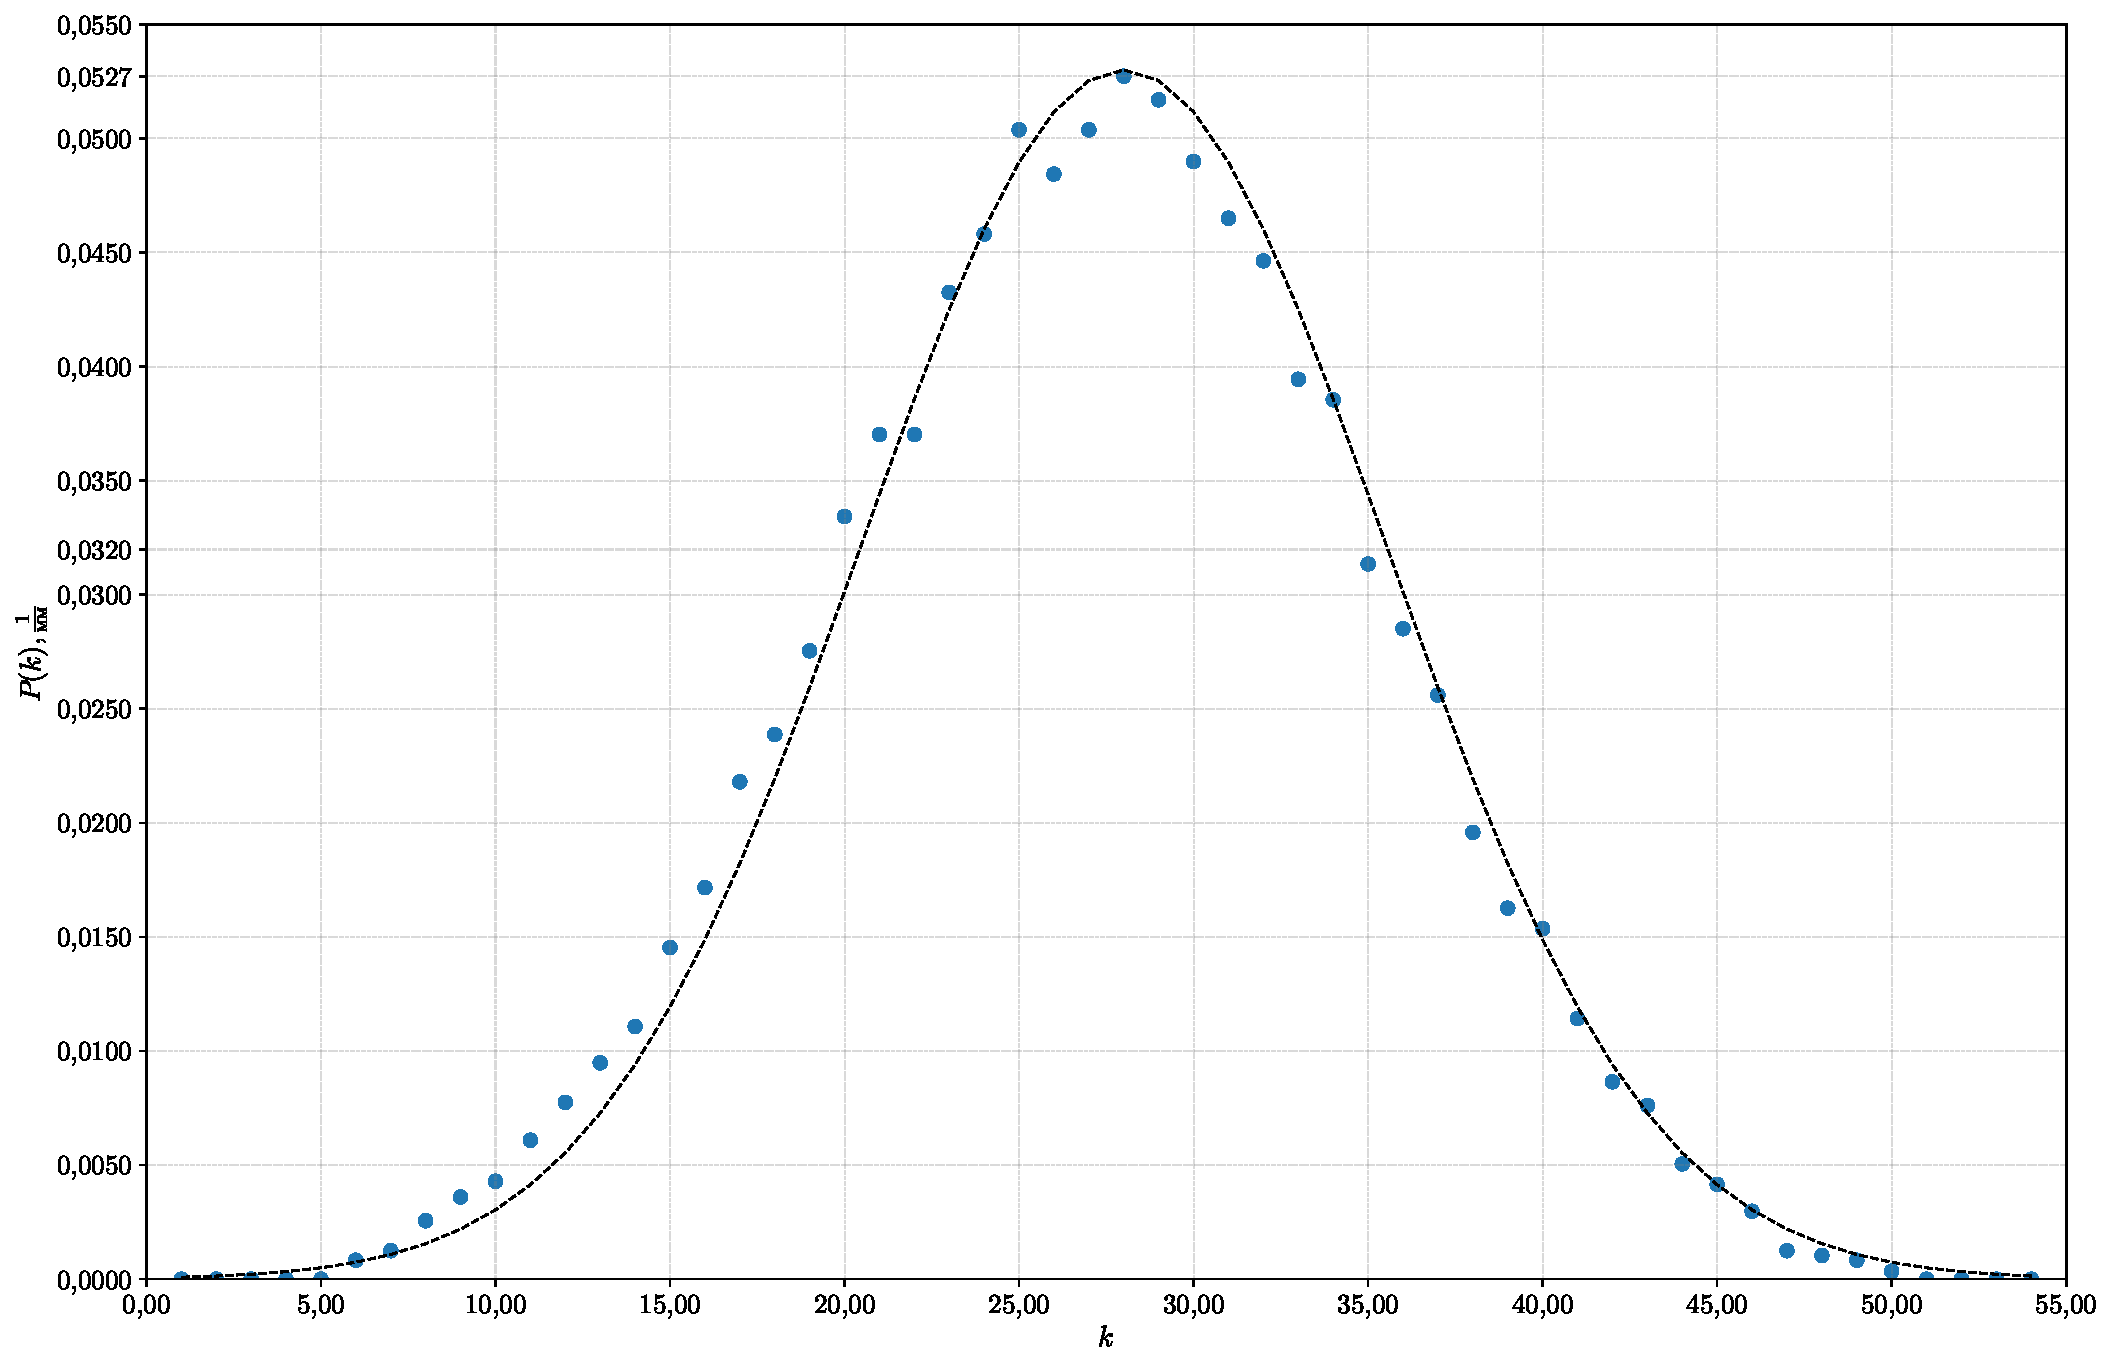
\includegraphics[angle = 270, width=0.8\textwidth]{ graph_1 } 
	\caption{График для $N = N_0/2$}
	
	 \label{fig:graph-1}
\end{figure}

\begin{figure}[H] 
	\centering
	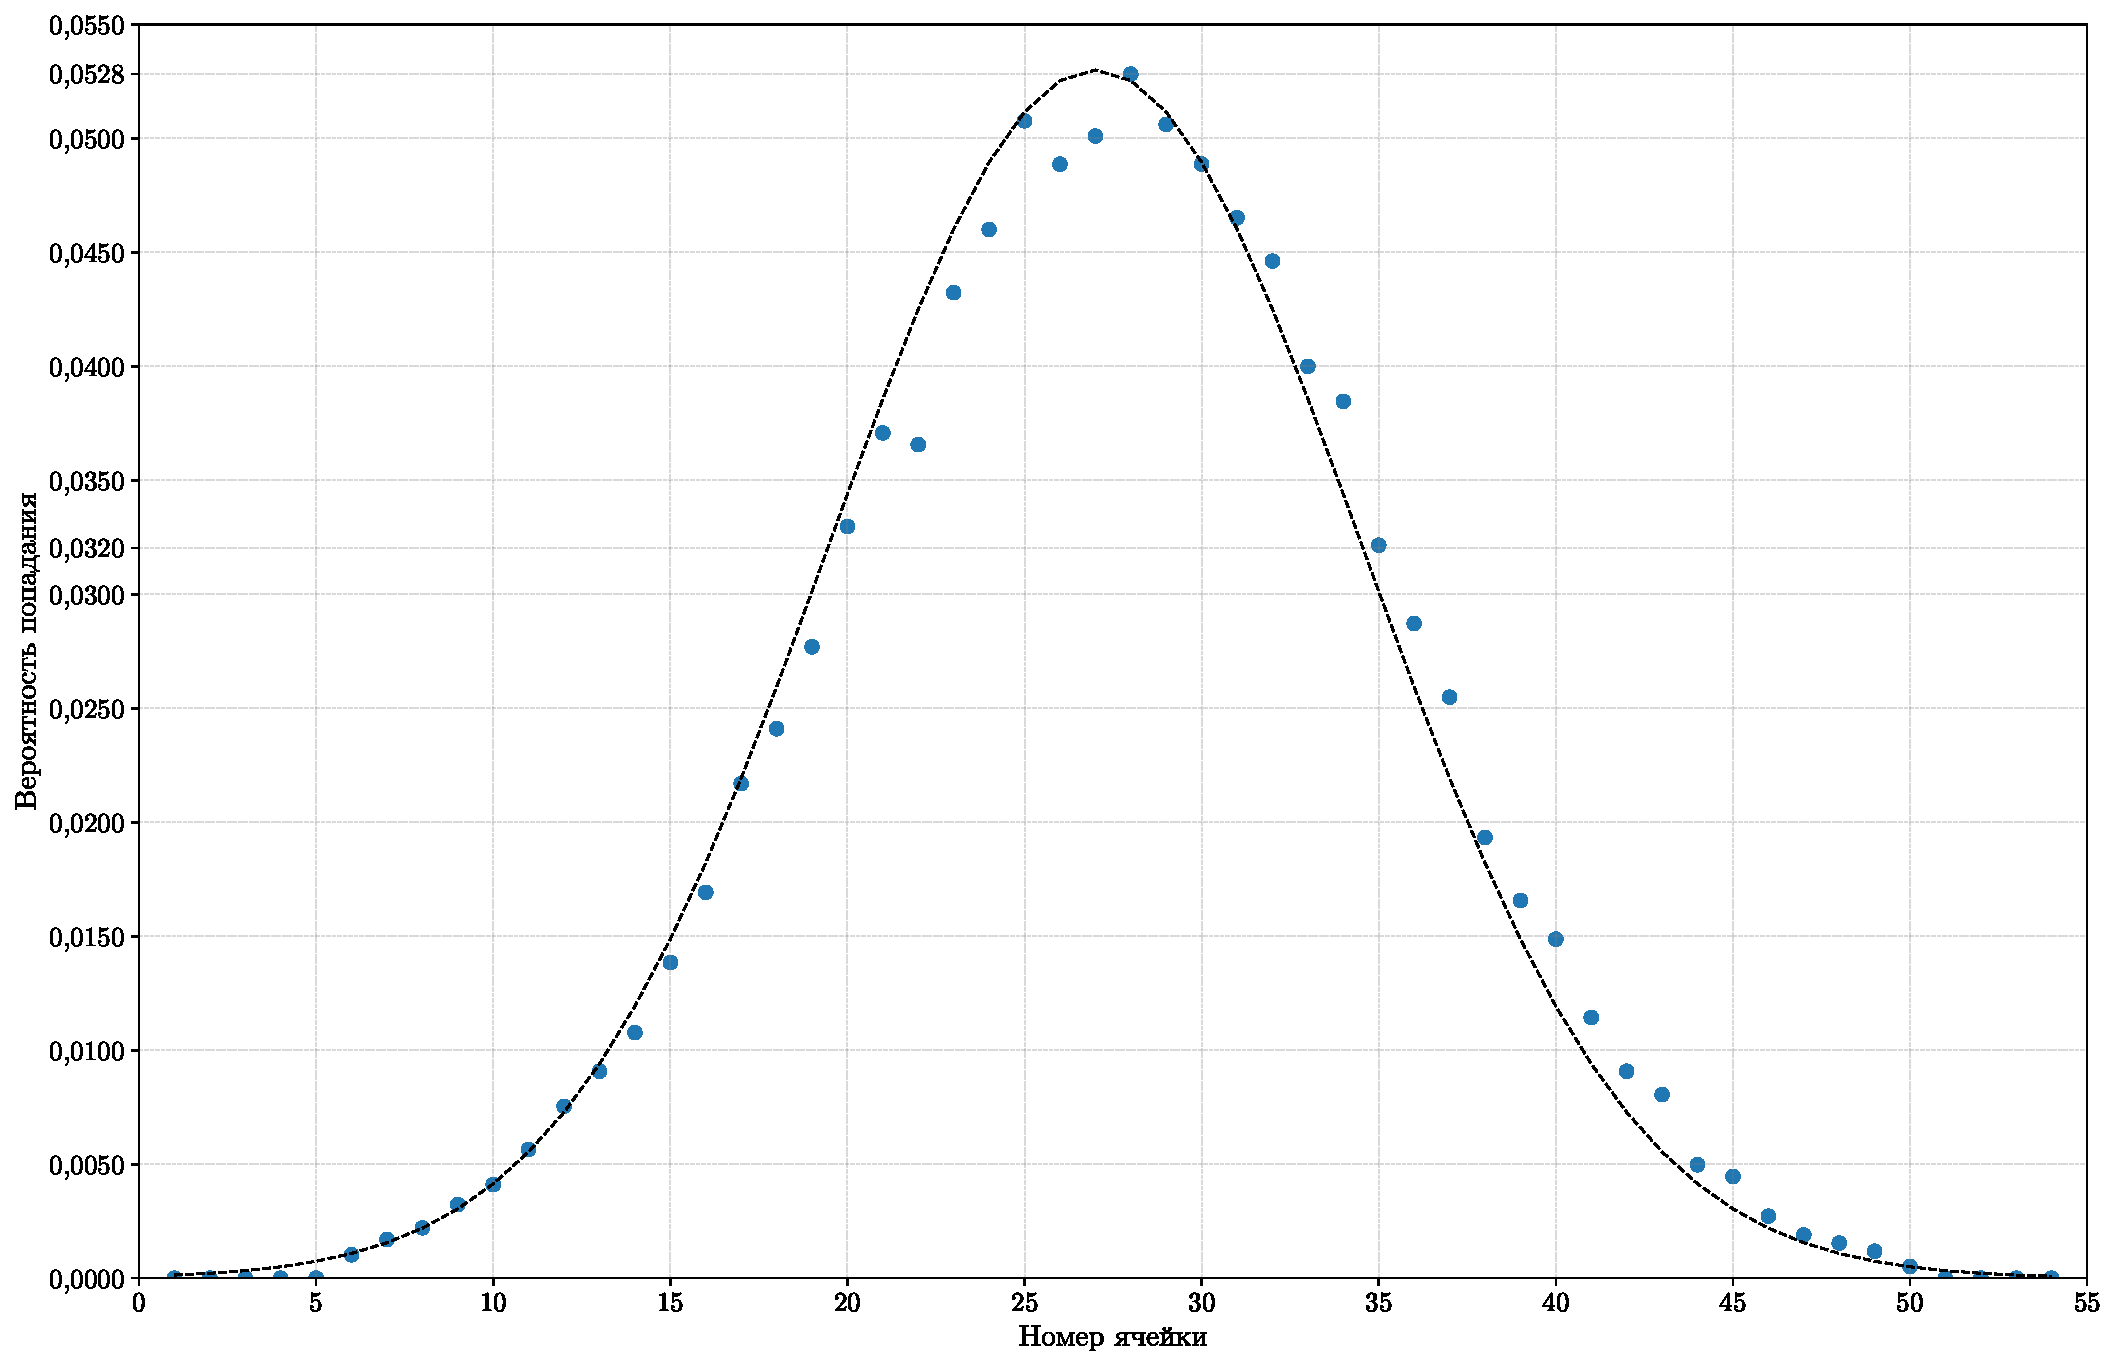
\includegraphics[angle = 270, width=0.8\textwidth]{ graph_2 } 
	\caption{График для $N = N_0$}
	
	\label{fig:graph-2} 
\end{figure}

\begin{figure}[H] 
	\centering
	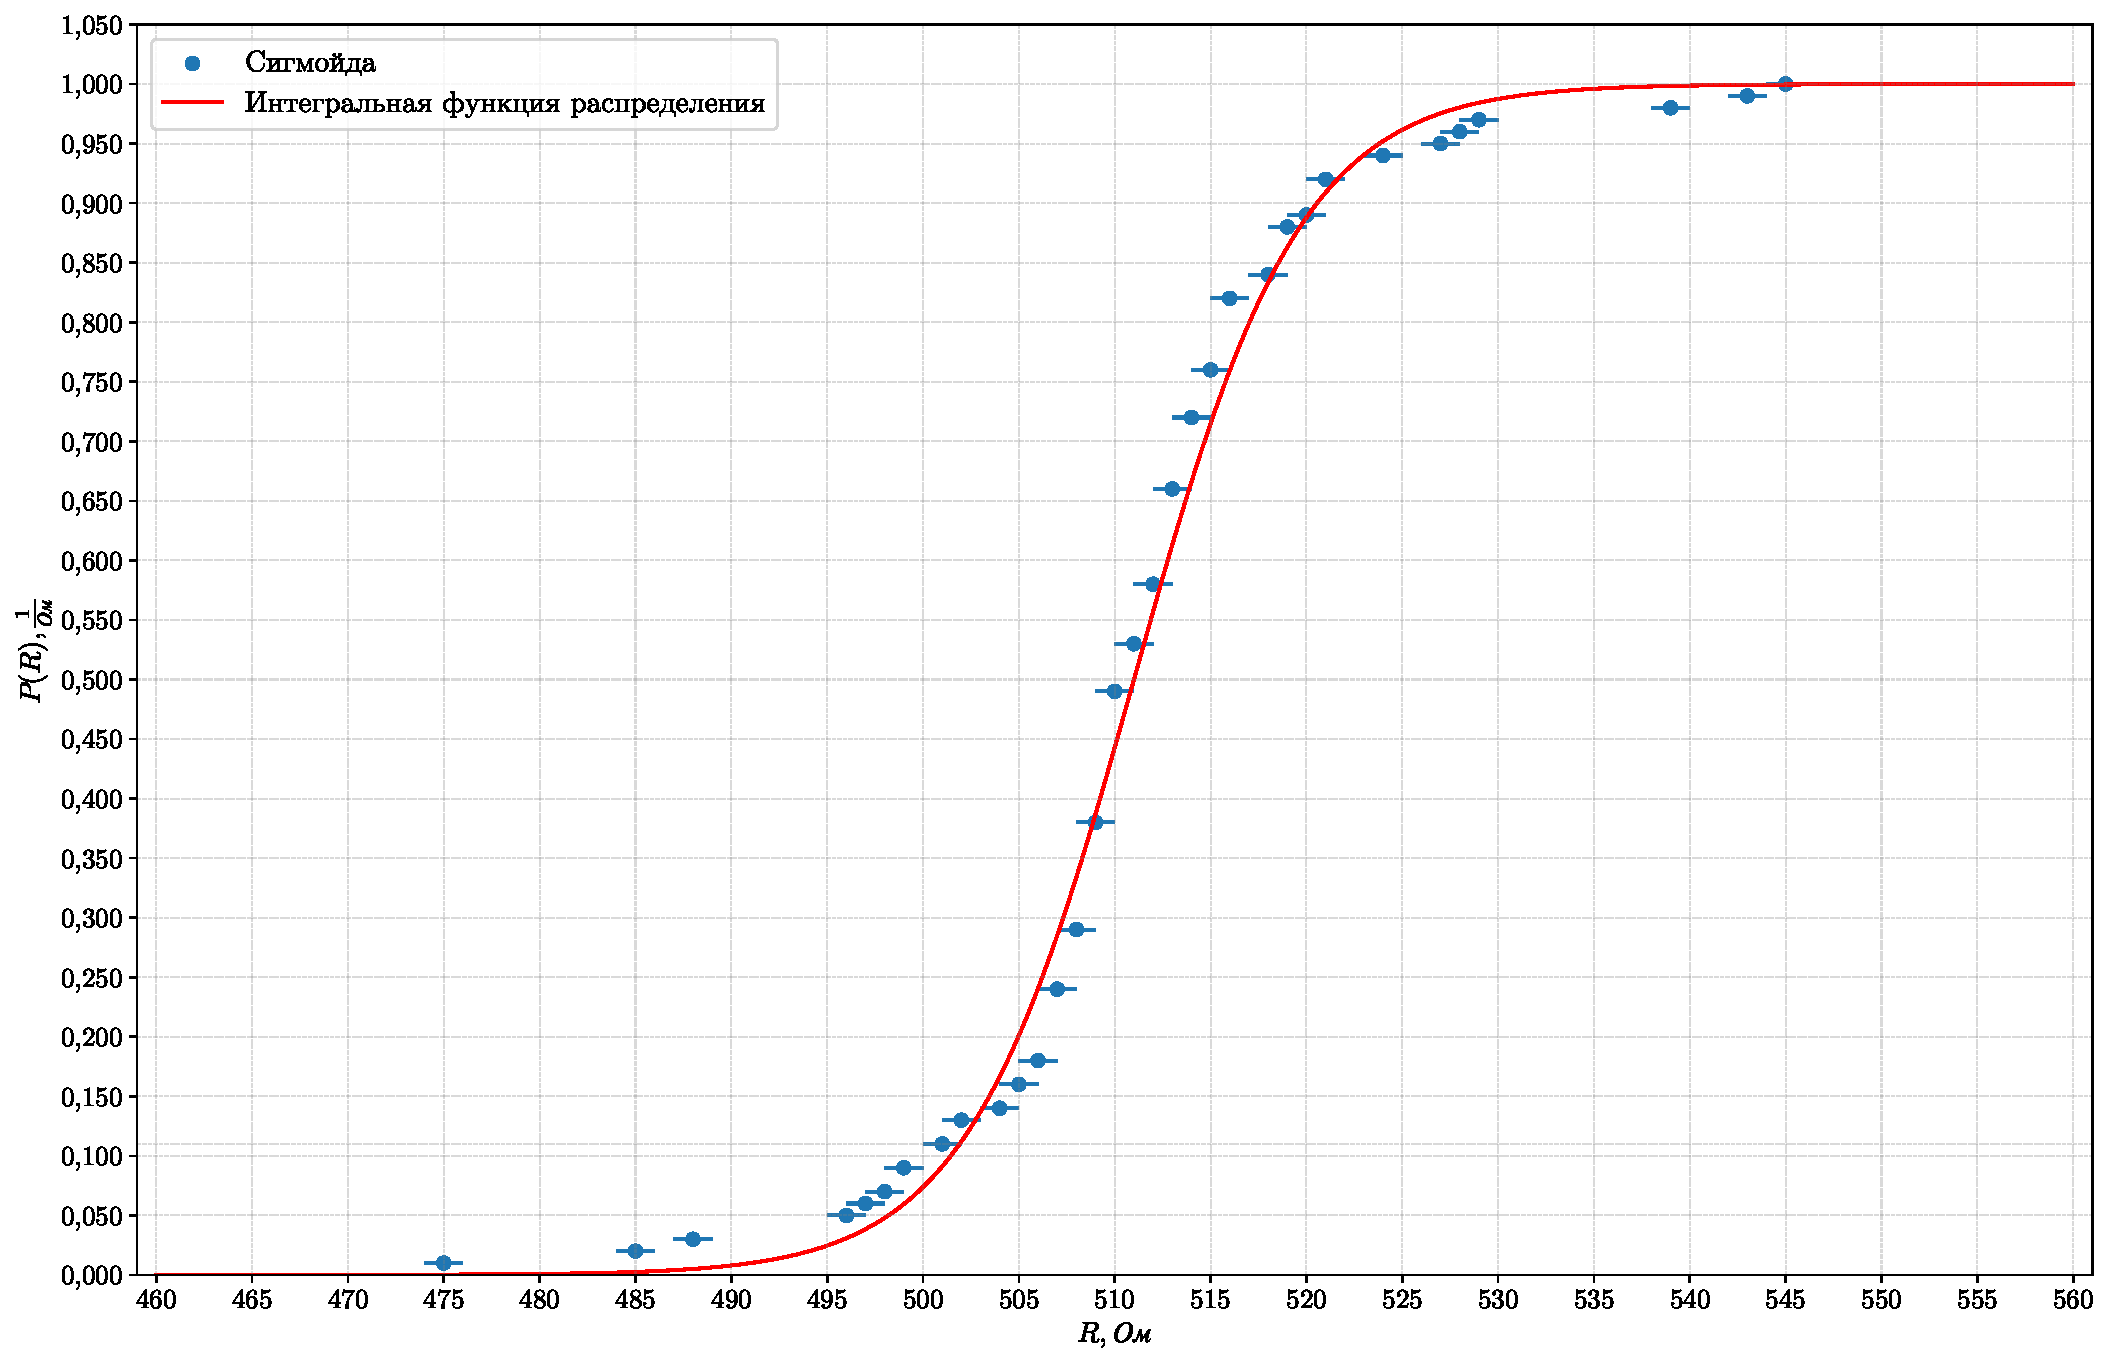
\includegraphics[angle = 270, width=0.8\textwidth]{ graph_3 } 
	\caption{График для опыта с резисторами $F(r)$}
	
	\label{fig:graph-3} 
\end{figure}

\begin{figure}[H] 
	\centering
	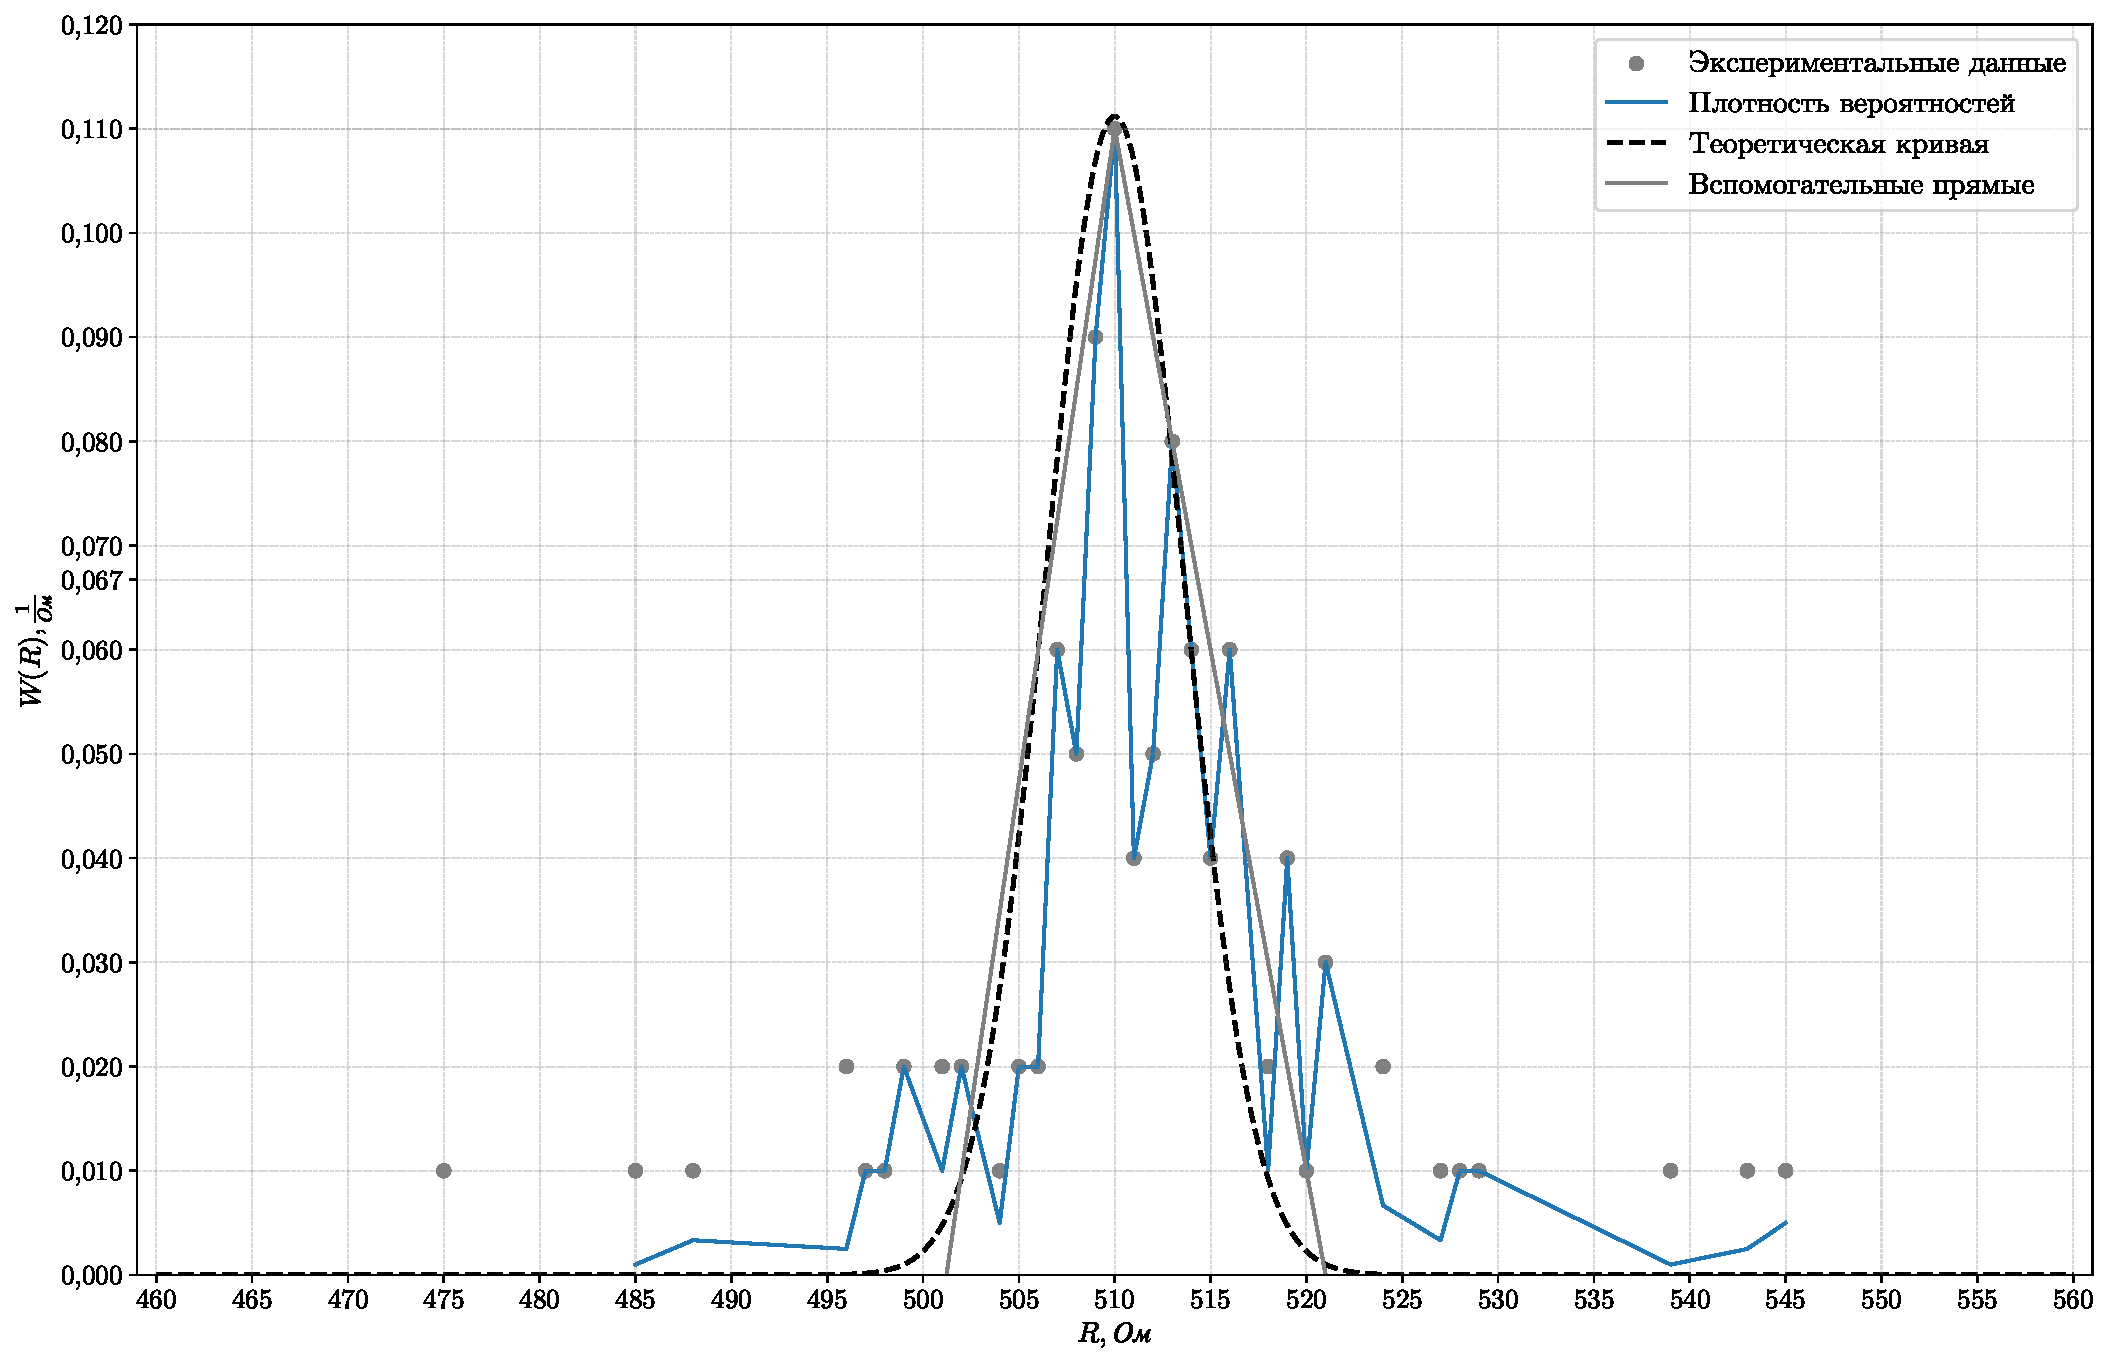
\includegraphics[angle = 270, width=0.8\textwidth]{ graph_4 } 
	\caption{График для опыта с резисторами (общий вид)}
	
	\label{fig:graph-4} 
\end{figure}

\end{document}